\chapter{Hintergrund} \label{cha:background}

\section{Containervirtualisierung}

Containervirtualisierung (auch Containerisierung genannt) beschreibt das Bereitstellen einer Applikation und deren Abhängigkeiten ((System-)Bibliotheken, ausführbare Dateien, (System-)Konfigurationen, etc.) als eine Einheit in Form eines "Container-Images". Das ermöglicht es, die Applikation isoliert, schnell und zuverlässig auf unterschiedlichen Host-Systemen auszuführen. Die einzige Anforderung an das Host-System ist dabei eine funktionierende Container-Laufzeitumgebung (z. B. Docker, Apptainer, Portainer, etc.).

Im Gegensatz zur klassischen Hardwarevirtualisierung wird bei der Containervirtualisierung nicht die Hardware-Ebene abstrahiert und ein komplett eigenständiges Betriebssystem hochgefahren, sondern lediglich die Betriebssystem-Ebene abstrahiert.

Das hat zur Folge, dass Containervirtualisierung in der Regel weniger Speicher verbraucht und performanter im Vergleich zu Hardwarevirtualisierung ist. \todo{Zitat}

\section{OCI-Container-Image Spezifikation}

Die Open Container Initiative (OCI) ist eine Organisation, welche sich auf die Standardisierung von Containern spezialisiert hat. Mitglieder dieser Initiative sind u. A. Microsoft, Amazon Web Services, Google und Red Hat. Die von OCI bereitgestellte Spezifikation definiert den Aufbau eines Container-Images. OCI-kompatible Container-Images können von unterschiedlichen Containervirtualisierungs-Lösungen ausgeführt werden, welche die OCI-Spezifikation unterstützen. Dazu zählen unter anderem Docker, ContainerD und Podman.

\section{ContainerD}

ContainerD ist ein System-Daemon, welcher die OCI-Image-Spezifikation unterstützt und die Verwaltung von Containern übernimmt. Docker nutzt ContainerD als Backend für die Containervirtualisierung. Das Unternehmen, welches hinter Docker steht, hat ContainerD initial entwickelt und später als Open-Source-Projekt veröffentlicht.

\begin{figure}[H]
    \includegraphicsWeb[width=\linewidth]{https://containerd.io/img/architecture.png}
    \captionof{figure}{ContainerD Architektur: https://containerd.io/img/architecture.png}
    \label{fig:containerd-architecture}
\end{figure}


ContainerD selber ist in mehrere Komponenten aufgeteilt. Der Aufbau von ContainerD, kann aus der \cref{fig:containerd-architecture} entnommen werden. Diese beinhalten unter anderem:

Eine API um mit unterschiedlichen ContainerD-Clients (Frontends) zu kommunizieren. Hierzu zählen CRI und die native ContainerD-Schnittstelle. CRI ist selber nur ein Wrapper um die native ContainerD-Schnittstelle. Die CRI-Schnittstelle wird größtenteils von Kubernetes genutzt, um ContainerD für die Containerverwaltung zu verwenden. Die native ContainerD-Schnittstelle wird unter anderem von Docker genutzt.

Der ContainerD-Core, welcher alle nötigen Metadaten und Funktionalitäten bereitstellt, um Container zu verwalten. Dieser kommuniziert wiederum mit dem ContainerD-Backend.

Das ContainerD-Backend ist für die eigentliche Ausführung der Container zuständig. Es abstrahiert die dafür nötigen Betriebssystem-Funktionalitäten für den ContainerD-Core. Diese Abstraktionen müssen durch einen sogenannten "Shim" implementiert werden. Der Shim ist ein kleines, plattformspezifisches Programm. Runc und d-shim sind Beispiele für Shims, welche auf Linux laufen. Runhcs wiederum ist ein Shim, welches auf Windows läuft und Windows-Container unterstützt.  

ContainerD benötigt erweiterte Rechte auf dem Host-System. Aus diesem Grund läuft ContainerD standardmäßig als Root-Prozess. Es ist mittlerweile auch möglich ContainerD als unprivilegierten Nutzer auszuführen. Dafür sind allerdings einige Systemkonfigurationsschritte notwendig, welche das Ausführen von ContainerD mit einem unprivilegierten Nutzer erschweren.

\pagebreak

\section{Docker}

Docker ist eine der am weitesten verbreiteten Containervirtualisierungslösungen \cite{LeadingContainerizationTechnologiesa}. Es beinhaltet eine Reihe von Werkzeugen zum Erstellen, Verwalten und Ausführen von Containern. Docker ist ein Frontend für ContainerD.

\subsection{Dockerfile}

Eine Dockerfile ist die Definition, welche Docker benötigt, um ein Container-Image zu erstellen. In dieser Datei werden alle nötigen Schritte sowie Metainformation definiert, um einen Container mit einer lauffähigen Applikation zu erstellen. Die in der Dockerfile definierten Schritte werden isoliert auf einem Basis-Image ausgeführt. Das durch die Dockerfile erstelle Image ist somit das Resultat aller Schritte, welche das Basis-Image darstellen und den Schritten, die in der Dockerfile definierten wurden \cite{dockerDockerfileOverview}.

In \cref{lst:dockerfile-example} ist ein simples Dockerfile Beispiel, welches ein Container-Image erstellt, was "Hello, Docker" mit cowsay ausgibt.

\begin{listing}[H]
    \caption{Dockerfile Beispiel}
    \label{lst:dockerfile-example}
    \inputminted{docker}{./code-examples/Dockerfile.example}
\end{listing}


\subsection{OCI-Container-Image Layer}

Ein OCI-Container-Image besteht aus Schichten (Layer), welche stapelweise angeordnet sind. In jeder Schicht werden Änderungen an der vorherigen Schicht vorgenommen. 

Jedes OCI-Container-Image hat die gleiche erste Schicht. Diese heißt "scratch". Auf dieser Schicht wird in der Regel eine spezifische Linux-Distribution aufgebaut. Ein Container-Image, welches nur ein Betriebssystem innehält, wird in der Regel als Grundlage für die Erstellung von Applikations-Container-Images verwendet. Aus diesem Grund nennt man solche Container-Images "Base image". Übliche Basis-Images sind z. B. Ubuntu, Debian und Alpine. 

Es ist unüblich, dass man bei der Containerisierung einer Applikation mit dem "scratch"-Layer startet. Stattdessen startet man mit einem bereits existierenden Basis-Image.

\subsection{Docker Build-Cache} \label{sec:bg-docker-cache}

Docker verfügt über Caching-Mechanismen, welche nachfolgende Builds beschleunigen \cite{dockerCache}. Das Caching funktioniert, indem Docker jedes einzelne "Layer" zwischenspeichert. Wenn sich die Definition eines Layers in der Dockerfile ändert, müssen nur die Layer, welche direkt oder indirekt auf dem Layer aufbauen, neu ausgeführt werden. 

Um das Caching von Docker möglichst effektiv zu verwenden, sollte man also sicherstellen, dass Layer, welche besonders lange zum Erstellen brauchen, möglichst nur dann neu erstellt werden, wenn dies tatsächlich notwendig ist.

Das heißt, dass besonders lange Schritte, wie z. B. das Kompilieren von Abhängigkeiten, möglichst weit oben in der Dockerfile definiert werden sollten. So wird sichergestellt, dass nur die Schritte von dem der besonders lange Schritt abhängt Einfluss, auf dessen erneute Ausführung haben.

\subsection{Docker BuildKit}

Docker BuildKit ist das neue Backend um OCI-Container-Images mit Docker zu erstellen. Ziel von BuildKit ist es, den Docker Legacy Builder zu ersetzen \cite{dockerBuildKit}.

Docker BuildKit hat viele Verbesserungen, um Docker-Builds im Vergleich zum Docker Legacy Builder performanter zu machen. Dazu zählen: Parallelisierung von Build-Stages, Auslassen von unbenutzten Build-Stages, mehr Caching Möglichkeiten wie z. B. Cache-Mounts, u. v. m.

Docker BuildKit Backends müssen nicht explizit auf dem Computer installiert werden, auf dem man entwickelt. Docker kann auch BuildKit Backend von Remote-Servern einbinden. Das ermöglicht es, Builds auf leistungsstärkeren Servern, sowie auf Servern mit einer anderen CPU-Architektur auszuführen, um die Build-Zeit zu verkürzen.

\subsubsection{Docker Buildx}

Um das Docker BuildKit Backend mit Docker vollwertig zu verwenden, nutzt man Docker Buildx \cite{dockerDockerBuildx}. Docker Buildx ist eine offizielle Docker Erweiterung. Docker Buildx hat einige Funktionalitäten um Docker BuildKit Backends einzubinden, sowie festzulegen welche BuildKit Backends man verwenden möchte.

\subsubsection{Docker Buildx Bake}

Eine weitere Funktionalität von Docker Buildx ist Docker Buildx Bake \cite{dockerBake}. Docker Buildx Bake ermöglicht es mithilfe einer sogenannten Bakefile das Erstellen mehrerer OCI-Container-Images zu vereinfachen.

Momentan wird JULEA in mehreren Ubuntu-Versionen sowie mit mehreren Kompilierern kompiliert und getestet. Somit müssten mehrere Dockerfiles erstellt werden, um alle Kombinationen für die Tests bereitzustellen. Mit Docker Buildx Bake kann man das Erstellen dieser großen Anzahl an Variationen von Docker-Container-Images in einer standardisierten Art und Weise definieren und mithilfe von Docker Buildx erstellen lassen. 

In \cref{lst:docker-bake-example} ist ein extensives Beispiel für eine Docker Buildx Bakefile.

\begin{listing}[H]
    \caption{Docker Buildx Bakefile Beispiel}
    \label{lst:docker-bake-example}
    \inputminted{./lexers/docker-bake-lexer.py}{./code-examples/docker-bake.example.hcl}
\end{listing}

\section{Container-Images für Entwicklungsumgebungen} \label{sec:bg-dev-container}

Während sich die klassische Containerisierung darauf fokussiert, eine produktive Applikation zuverlässig auszurollen, fokussieren sich Container-Images für Entwicklungsumgebungen darauf, Entwicklern eine einheitliche Container-Umgebung zum Testen und Entwickeln einer Applikation bereitzustellen. Im Idealfall sollte ein Entwicklungs-Container den Einstieg für neue Entwickler in ein Projekt erleichtern, indem dieser eine bereits vorkonfigurierte Entwicklungsumgebung bereitstellt.

Solche Container-Images sollten alle nötigen Abhängigkeiten, welche man zum Entwickeln benötigt, enthalten. Dazu zählen z. B. Compiler, Interpreter, Bibliotheken, Tools.

Im Fall von JULEA muss ein solcher Entwicklungs-Container alle Abhängigkeiten enthalten, um an oder mit JULEA zu entwickeln. Diese Abhängigkeiten müssen kompiliert werden. Das Kompilieren ist sehr zeitaufwendig. Darum sollte ein fertiges Container-Image diese Abhängigkeiten beinhalten, sodass das initiale Kompilieren der Abhängigkeiten durch den Entwickler übersprungen werden kann.

Ein Container-Image alleine müsste allerdings immer noch vom Entwickler selbst in den Editor/IDE integriert werden, da das Benutzen des Containers ohne eine solche Integration mit mehr Aufwand verbunden wäre. Um die Integration in den Editor/IDE zu vereinfachen und zu standardisieren, bietet Microsoft eine offene Spezifikation ("Development Container") an \cite{DevelopmentContainers}. Wenn ein Editor/IDE diese Spezifikation unterstützt und ein Projekt eine Development Container Konfiguration erstellt hat, kann der Entwickler mit einem Klick den Container in den Editor/IDE integrieren und wie gewohnt mit dem Projekt arbeiten.

Neben der einfachen Integration eines Containers in den Editor/IDE bietet die Development-Container-Spezifikation eine Reihe an Einstellungsmöglichkeiten an. So kann man z. B. festlegen, welche Extensions installiert werden sollen, welche Umgebungsvariablen gesetzt werden sollen, welche Ports nach außen freigegeben werden sollen, welche Editor/IDE-Einstellungen gesetzt werden sollen, u. v. m.

\pagebreak

\subsection{Editor/IDE-Unterstützung}

In \cref{tbl:editor-ide-support} ist eine Übersicht über die aktuelle Editor/IDE-Unterstützung der Development-Container-Spezifikation.

\begin{table}[H]
    \caption{Devcontainer Spezifikation Editorunterstützung}
    \label{tbl:editor-ide-support}
    \begin{tblr}{colspec={|X[3]|X[2]|X[6]|}, hlines, width=\linewidth}
        IDE/Editor Name    & Unterstützung & Anmerkung \\
        Visual Studio Code & Ja            & vollständige Unterstützung                                                                                                                                                                                              \\
        CLI                & Ja            & Es existiert ein offizielles CLI in Form eines NPM-Paketes @devcontainer/cli. Dadurch ist es auch möglich \(Neo-\)VIM und andere Terminal-Texteditoren mit Devcontainern zu verwenden                                   \\
        Visual Studio      & Ja*           & Stand 01.12.2024: eingeschränkte Unterstützung. Aktuell sind nur C++-Projekte mit CMake unterstützt                                                                                                                      \\
        JetBrains IDEs     & Ja*           & Stand 01.12.2024 ist die Unterstützung in der Beta-Phase und unvollständig.                                                                                                                                             \\
        VIM                & Ja*           & Stand 01.12.2024 gibt es ein Community-Plugin für Neo-VIM welches Devcontainer-Integration ermöglicht. Die Vollständigkeit dieses Plugins wurde nicht überprüft. Siehe: https://codeberg.org/esensar/nvim-dev-container \\
        Sublime Text       & Nein          & Stand 01.12.2024: Es gibt keine offizielle Aussage, ob oder wann es eine Devcontainer-Unterstützung geben soll                                                                                                            \\
        Eclipse            & Nein          & Stand 01.12.2024: Es gibt keine offizielle Aussage, ob oder wann es eine Devcontainer-Unterstützung geben soll                                                                                                            \\
        Netbeans           & Nein          & Stand 01.12.2024: Es gibt keine offizielle Aussage, ob oder wann es eine Devcontainer-Unterstützung geben soll                                                                                                            \\
        Code::Blocks       & Nein          & Stand 01.12.2024: Es gibt keine offizielle Aussage, ob oder wann es eine Devcontainer-Unterstützung geben soll                                                                                                            \\
        Notepad++          & Nein          & Stand 01.12.2024: Es gibt keine offizielle Aussage, ob oder wann es eine Devcontainer-Unterstützung geben soll                                                                                                            \\
        Emacs              & Nein          & Stand 01.12.2024: Es gibt keine offizielle Aussage, ob oder wann es eine Devcontainer-Unterstützung geben soll                                                                                                            \\
\end{tblr}
\end{table}


\section{Apptainer (früher: Singularity)} \label{sec:bg-apptainer}

Apptainer ist eine alternative Container-Lösung. Apptainer nutzt im Gegensatz zu Docker keine OCI-Container-Images, kann allerdings OCI-Container zu Apptainer-Container konvertieren. Apptainer-Container-Images werden als einzelne Datei gespeichert, das erleichtert das Verteilen von Container-Images ohne einen dedizierten Registry-Server. 

Im Gegensatz zu einer üblichen ContainerD-Installation werden keine erweiterten Berechtigungen durch Apptainer benötigt, um Container auszuführen. Dies ist insbesondere für HPC-Umgebungen relevant, da das Ausführen von Applikationen als root-Benutzer hier ungewöhnlich ist \cite{apptainerApptainerPortableReproducible}. 

Außerdem hat Apptainer eine extensive Dokumentation, wie man MPI mit Apptainer nutzen kann, was für HPC-Umgebungen von Relevanz ist \cite{apptainerApptainerMPIApplications}. 

Ein weiteres wichtiges Merkmal von Apptainer ist die weniger strikte Isolierung von Containern zum Host-System \cite{apptainerSecurityApptainerApptainer}, verglichen mit z. B. ContainerD. Das ermöglicht es u. A. unkompliziert auf spezielle Ressourcen, wie z. B. GPUs zuzugreifen, was in HPC-Umgebungen üblich ist. Zugriff auf GPUs ist mit Docker nur dann möglich, wenn man Docker entsprechend konfiguriert hat \cite{ResourceConstraints0200}.

\section{CI/CD-Pipeline} \label{sec:ci-cd-pipeline}

\begin{figure}[H]
    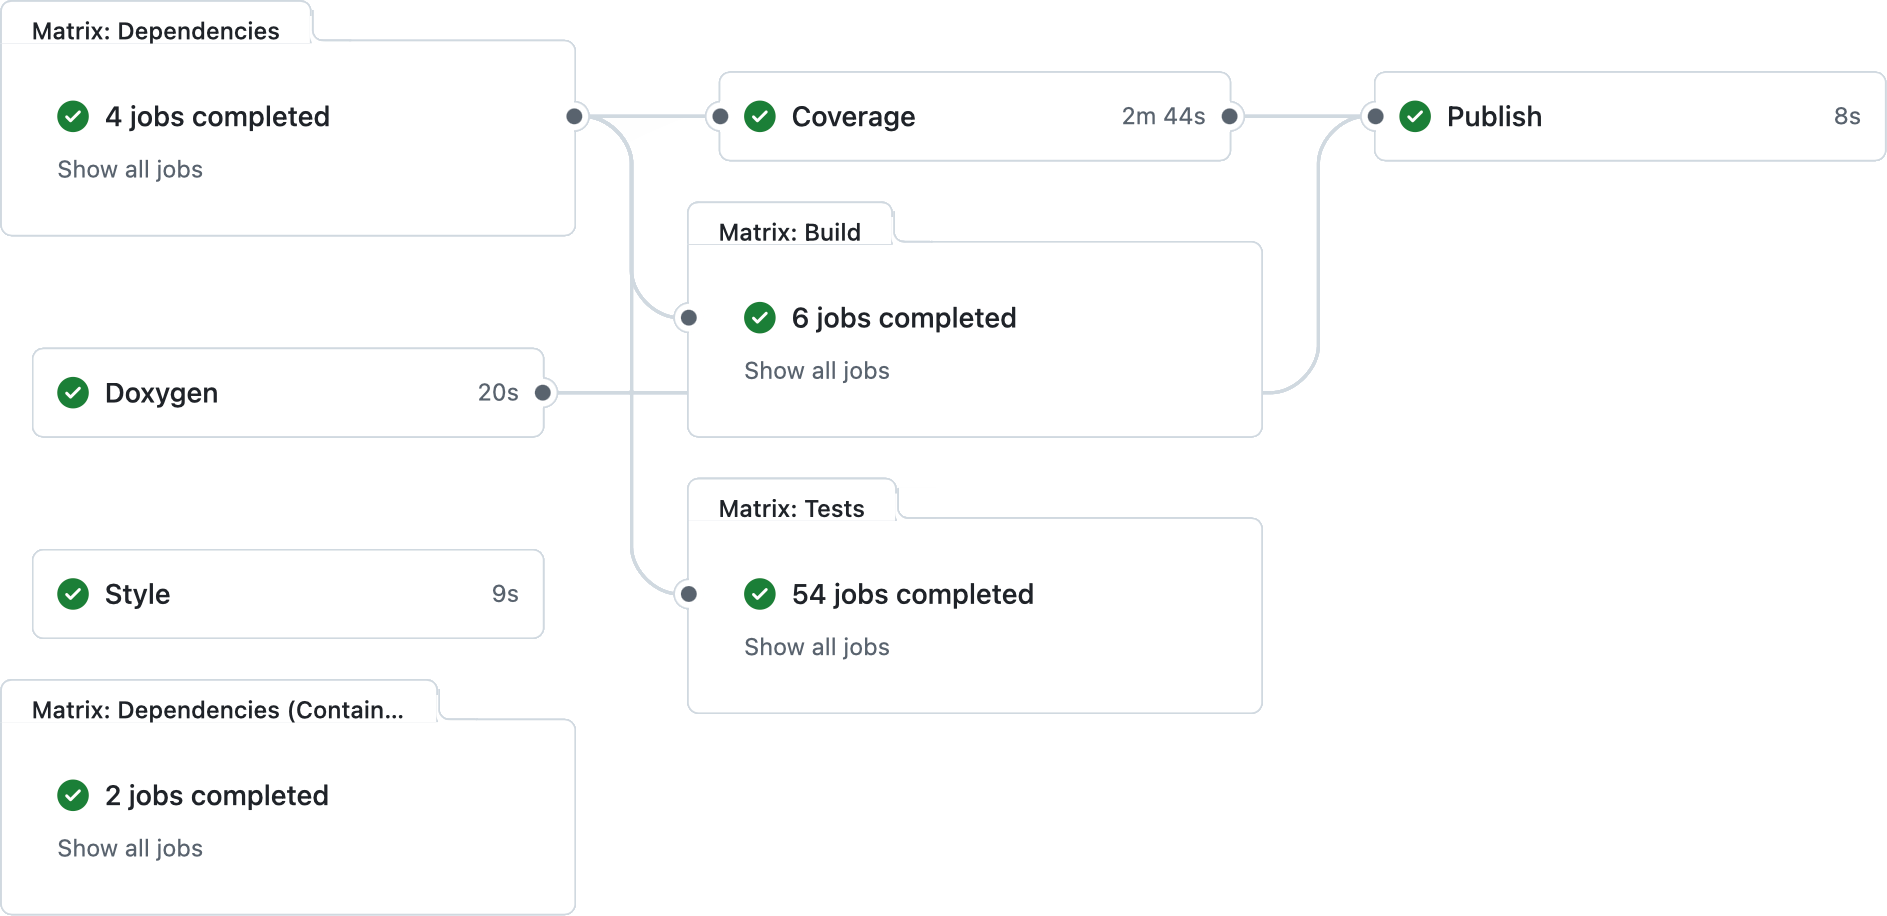
\includegraphics[width=\textwidth]{./figures/ci-julea-exmaple-full.png}
    \label{fig:ci-cd-julea-example-full}
    \caption{CI/CD-Pipeline von JULEA. \newline
        Siehe: https://github.com/parcio/julea/actions/runs/8318540808}
\end{figure}

CI/CD ist die Kombination von Continuous Integration (CI) und Continuous Deployment/Continuous Delivery (CD). Eine CI/CD-Pipeline ist eine automatisierte Ausführung der CI- und CD-Prozesse. Dies ist üblicherweise das automatisierte Testen von Applikationskomponenten, Kompilieren der Applikation, das Bereitstellen und Ausrollen von Artefakten. 

Oftmals sind solche CI/CD-Pipeline-Funktionalitäten direkt Teil einer modernen Version-Control-System-Plattform wie z. B. GitHub, GitLab, BitBucket, etc. und integrieren sich in das Version-Control-System der Platform, indem sie z. B. vollautomatisch auf Code-Änderungen reagieren können. 

In \cref{fig:ci-cd-julea-example-full} ist eine Visualisierung der bereits existierenden CI/CD-Pipeline von JULEA zu sehen. Man sieht mehrere Schritte, welche aufeinander aufbauen. Die Abhängigkeiten untereinander werden durch die Kanten, welche die einzelnen Schritte (Knoten) verbinden, dargestellt.


\pagebreak

\subsection{Continuous Integration (CI)}

Unter Continuous Integration (CI) versteht man alle Prozesse, welche die einzelnen Softwareteile kontinuierlich zu einer Software zusammenführt. Üblicherweise zählt dazu das regelmäßige Kompilieren und Testen einer Applikation.

Wie bereits in \cref{sec:ci-cd-pipeline} erwähnt, kann CI ein Teil der CI/CD-Pipeline sein.

Im gezeigten Beispiel gehören alle bis auf den letzten Schritt "Publish" zur Continuous Integration (CI).

\begin{figure}[H]
    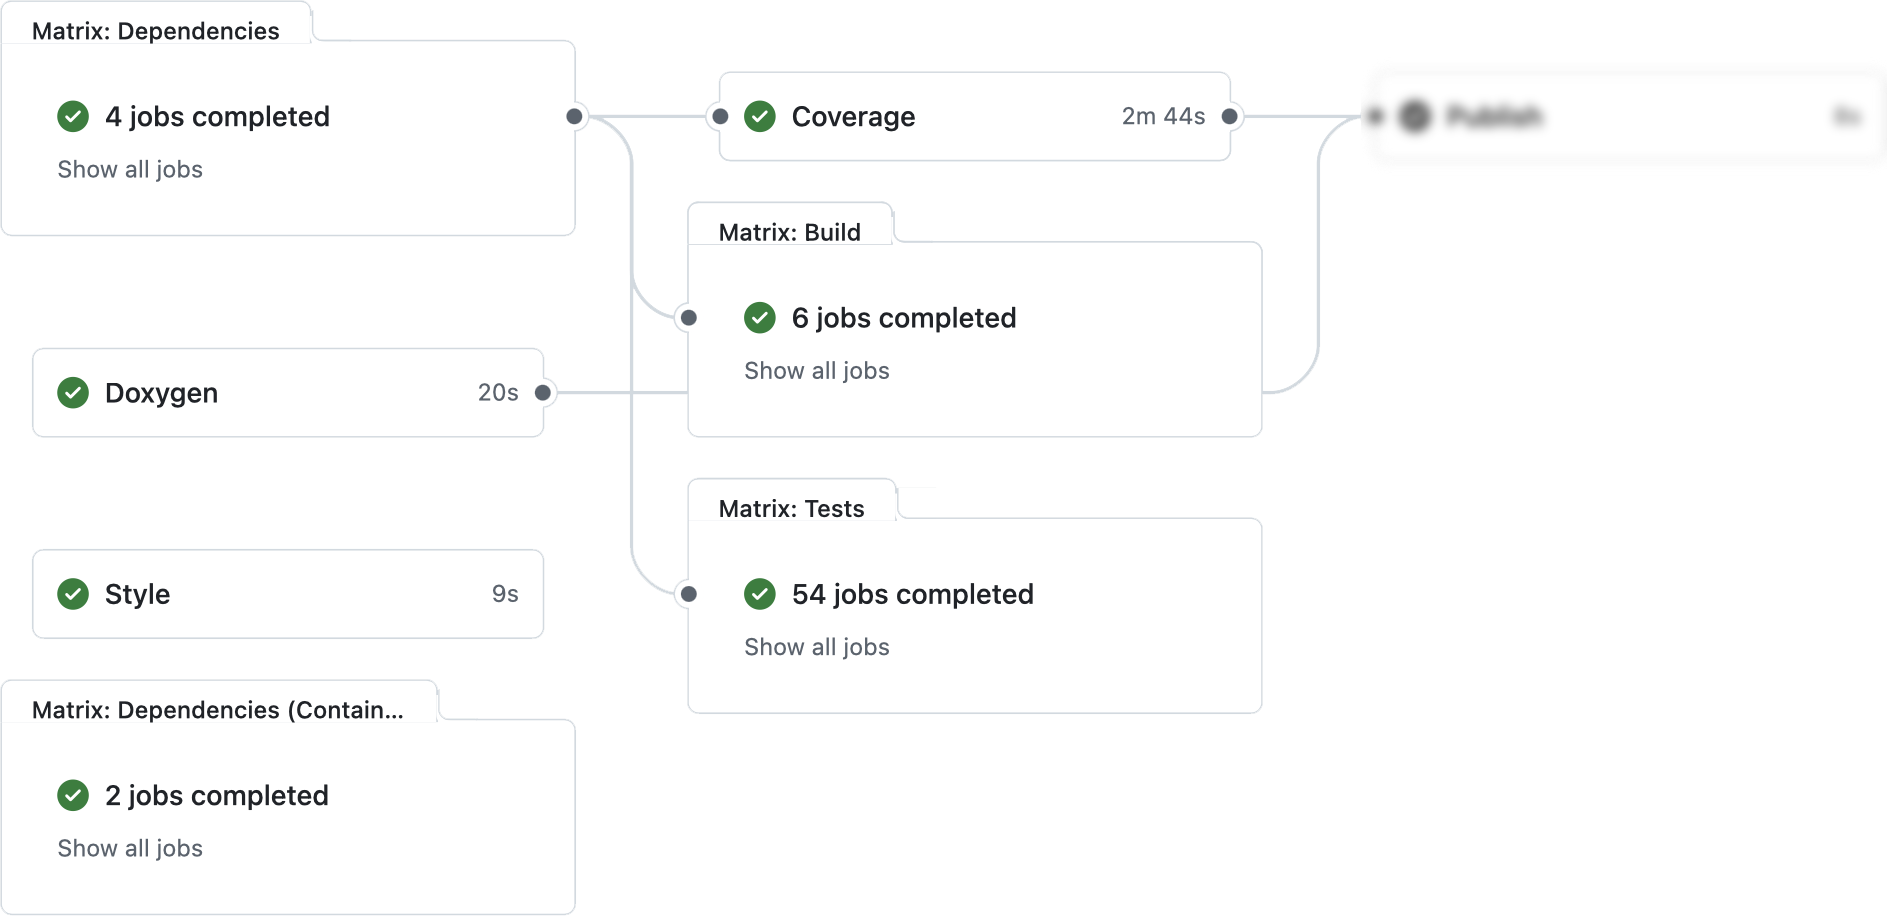
\includegraphics[width=\textwidth]{julea-ci-cd-ci-focus.png}
    \caption{CI/CD-Pipeline von JULEA. \newline
        Siehe: https://github.com/parcio/julea/actions/runs/8318540808}
\end{figure}

\pagebreak

\subsection{Continuous Delivery (CD)}

Continuous Delivery baut auf dem Konzept von Continuous Integration auf. Anstelle die Applikation nur zu kompilieren und zu testen, wird bei Continuous Delivery ein Artefakt bereitgestellt, sobald eine gewisse Qualität erreicht worden ist z. B. alle definierten Tests der Applikation erfolgreich waren. 

Continuous Delivery kann – wie bereits in \cref{sec:ci-cd-pipeline} erwähnt – ein Teil einer CI/CD-Pipeline sein. 

Im gezeigten Beispiel in \cref{fig:julea-ci-cd-cd-focus} macht der letzte Schritt "Publish" diese Pipeline erst zu einer Continuous-Delivery-Pipeline. Im genannten Schritt wird die Dokumentation von JULEA automatisch veröffentlicht. Hier ist allerdings zu erwähnen, dass die Veröffentlichung der Dokumentation nicht zwingend ein Release der Applikation bedeutet. Außerdem ist die Veröffentlichung der Dokumentation nicht abhängig von den ausgeführten Tests. 

Eine Continuous-Delivery-Pipeline – wie sie in diesem Abschnitt beschrieben ist – würde die Veröffentlichung der Dokumentation nur dann ausführen, wenn alle Tests erfolgreich waren und es würde neben der Dokumentation auch ein neues Release der Applikation veröffentlicht werden.

\begin{figure}[H]
    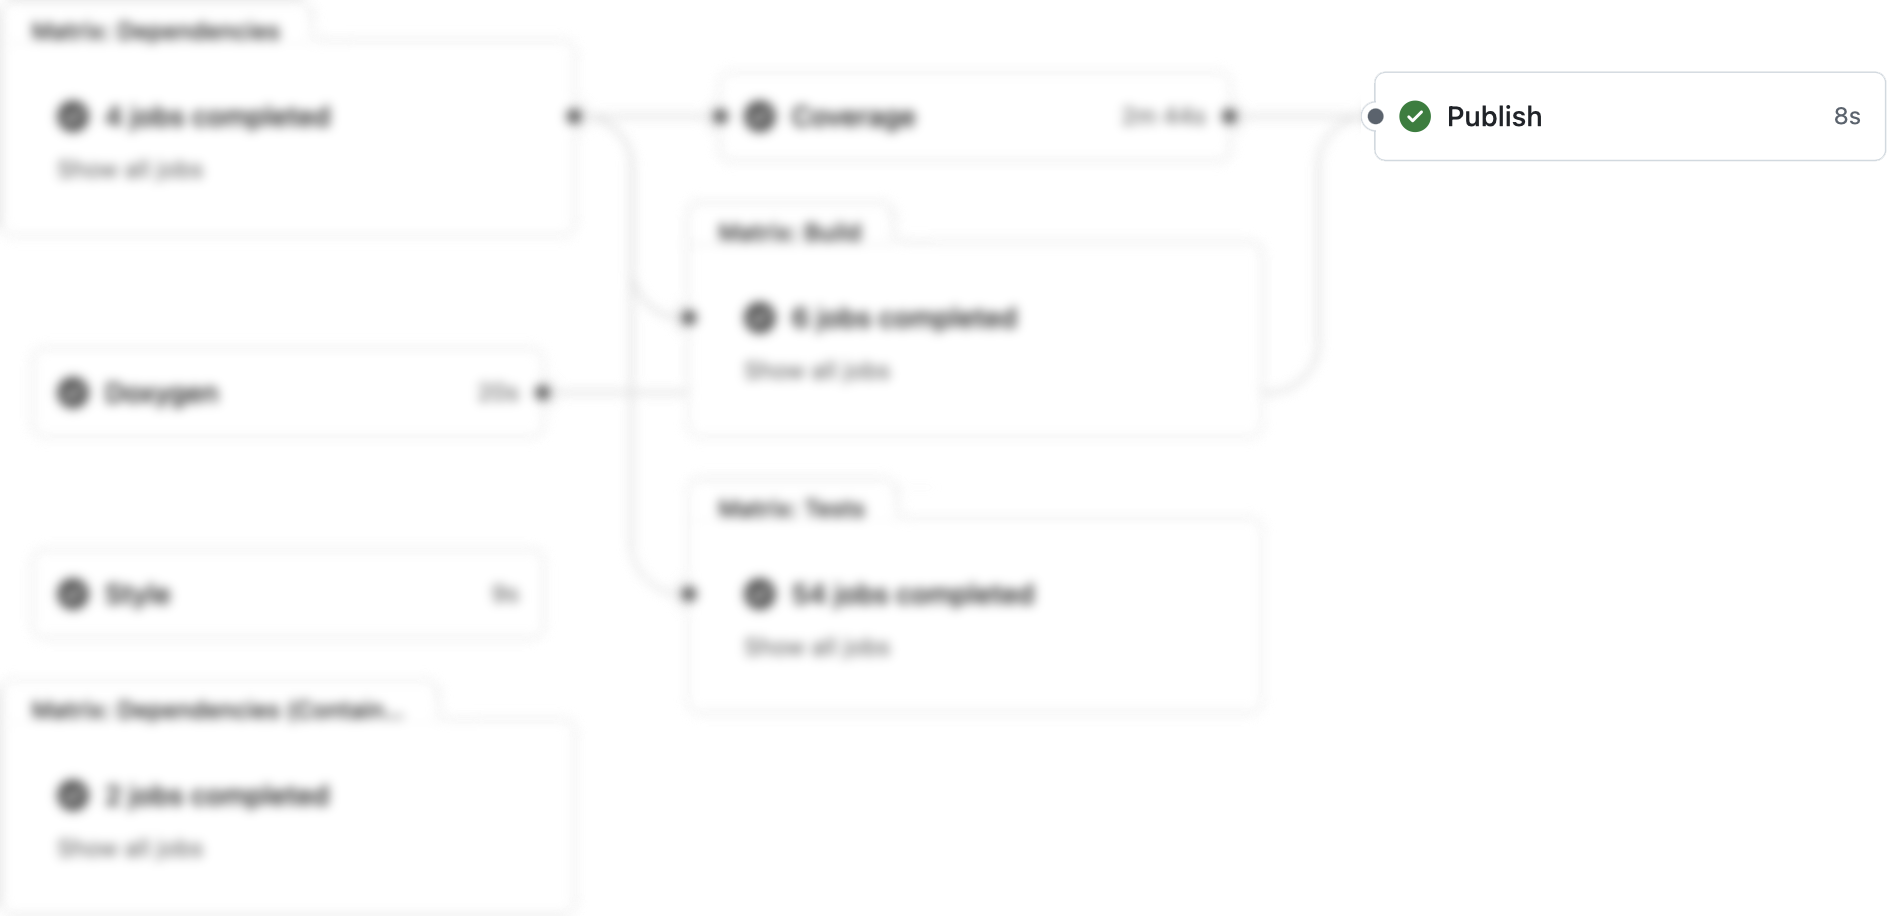
\includegraphics[width=\textwidth]{julea-ci-cd-cd-focus.png}
    \caption{CI/CD-Pipeline von JULEA. \newline
        Siehe: https://github.com/parcio/julea/actions/runs/8318540808}
    \label{fig:julea-ci-cd-cd-focus}
\end{figure}

\subsection{Continuous Deployment}

Continuous Deployment baut auf dem Konzept von Continuous Delivery auf. Anstelle Artefakte nur bereitzustellen, wird bei Continuous Deployment das bereitgestellte Artefakt auch auf das Produktivsystem ausgerollt.

Das automatisierte Ausrollen kann auch in mehreren Schritten durchgeführt werden, indem es zuerst in ein Staging-System ausgerollt wird. Erst nach einer problemfreien Testphase werden dann im Anschluss die Änderungen auf das Produktivsystem ausgerollt. 

Continuous Deployment kann – wie bereits in \cref{sec:ci-cd-pipeline} erwähnt – ein Teil einer CI/CD-Pipeline sein.

\subsection{GitHub-Actions}

GitHub-Actions (GHA) ist die GitHub-eigene CI/CD-Pipeline-Lösung. GitHub-Actions ermöglicht es mithilfe einer YML-Datei CI/CD-Pipelines zu definieren. Diese YML-Datei wird im Repository abgelegt und von GitHub-Actions ausgeführt. 

GitHub-Actions bietet eine Vielzahl von vordefinierten Funktionsbausteinen an. Diese Funktionsbausteine haben häufig in CI/CD-Pipelines benötigte Logiken schon vordefiniert und erleichtern somit das Erstellen von CI/CD-Pipelines. Diese Bausteine werden entweder von GitHub oder Dritten zur Verfügung gestellt. Die Bausteine werden in einer isolierten Container-Umgebung ausgeführt, um möglichst reproduzierbare Ergebnisse zu erzielen \cite{githubGitHubActions}.

GitHub-Actions wird in dieser Arbeit genutzt, um automatisiert die JULEA-Container-Images zu erstellen und zu veröffentlichen.

In \cref{lst:gha-example} wird eine beispielhafte GitHub-Actions-Workflow-Datei gezeigt. Diese Datei ist Teil der GitHub-Dokumentation \cite{githubSchnellstartFuerGitHub}

\begin{listing}[H]
    \caption{GitHub-Actions Beispiel}
    \label{lst:gha-example}
    \inputminted{yaml}{./code-examples/gha.yml}
\end{listing}


\section{JULEA}

In dieser Arbeit wird JULEA als Beispiel für eine Applikation verwendet, welche in einem Container-Image bereitgestellt werden soll. JULEA ist ein Speicher-Framework, welches mehrere Speicher-Backends wie z. B. Datei-Speicher, MySQL, MongoDB, u. v. m. unterstützt. JULEA soll das Testen von verschiedenen Speichertechnologien erleichtern, indem es eine einheitliche API bereitstellt, welche unabhängig von der unterliegenden Speichertechnologie ist. JULEA ist ein Open-Source-Projekt und wird unter anderem von der Arbeitsgruppe "Parallel Computing and I/O" an der Otto-von-Guericke-Universität Magdeburg entwickelt \cite{kuhnJULEAFlexibleStorage2017}.

Der Quellcode von JULEA wird auf GitHub bereitgestellt: \url{https://github.com/parcio/julea}

\section{HPC}

HPC steht für High Performance Computing. HPC-Systeme sind spezielle Computersysteme, die besonders leistungsstark sind. HPC-Systeme werden für Berechnungen mit besonders hohen CPU oder Speicheranforderungen genutzt. Oft finden HPC-Systeme in Forschungseinrichtungen, Universitäten, oder in der Industrie Gebrauch. HPC-Applikationen sind häufig hochkomplex und greifen auf große Mengen von Abhängigkeiten zurück, welche entweder zur Kompilierungszeit, oder zur Laufzeit benötigt werden. Eine hohe Anzahl an Abhängigkeiten erschwert das Erstellen von reproduzierbaren Laufzeit-, und Kompilierungsergebnissen, da die mögliche Kombination von Abhängigkeiten, welche zur Laufzeit und/oder zur Kompilierzeit benötigt werden, sehr hoch ist. 

Die Komplexität von Abhängigkeiten in einer Applikation lässt sich folgendermaßen modellieren:
\begin{flalign*}
    &\text{Sei } D_a = (x_0,\dots, x_n), x_i \in \mathbb{N} \\&
    \text{und } x_i \text{ die Anzahl der akzeptierten Variationen der }i\text{-ten Abhängigkeit der Applikation } a&
\end{flalign*}
dann ist die Anzahl der unterschiedlichen Umgebungen, in der die Applikation $a$ funktionieren sollte: 
\begin{align*}
   \prod_{i=0}^{|D_a|} x_i
\end{align*}

Angenommen, es gibt eine Applikation $b$, welche 3 Abhängigkeiten mit jeweils 3 akzeptierten Varianten hat ($D_b = (3, 3, 3)$), dann ist: 
\begin{align*}
    \prod_{i=0}^{|D_b|} x_i &= \prod_{i=0}^{3} x_i\\
    &= 3 \cdot 3 \cdot 3 \\
    &= 27
\end{align*}

Seien:
\begin{align*}
    f(n) &= (x_i)_{i=0}^{n}, \text{wobei } n \in \mathbb{N} \text{ und } x_i = 3 \\
    g(n) &= \prod_{i=0}^{|f(n)|} f(n)
\end{align*}

Dann stellt $g(n)$ die Anzahl der unterschiedlichen Umgebungen für $n$ Abhängigkeiten mit jeweils 3 akzeptierten Variationen je Abhängigkeit dar:

\begin{tikzpicture}
    \begin{axis}[
        axis lines = left,
        xlabel = \(n\),
        ylabel = {\(g(n)\)},
    ]
    %Below the red parabola is defined
    \addplot [
        domain=0:6,
        samples=100, 
        color=red,
    ]
    {3^x};
    \addlegendentry{\(\prod_{i=0}^{|f(n)|} f(n)\)}
    
    \end{axis}
\end{tikzpicture}

Es wird ersichtlich, dass die Anzahl der unterschiedlichen Umgebungen exponentiell mit der Anzahl der akzeptierten Abhängigkeiten (Variationen) wächst. 

Dies bedeutet, dass Applikationen, welche über sehr viele Abhängigkeiten mit sehr vielen Abhängigkeitsvariationen (Versionen, Kompilierung-Flags, etc.) verfügen schwer zu testen sind. Dies liegt daran, dass es so gut wie unmöglich ist, jede mögliche Umgebung mit jeder möglichen Applikationsvariante zu testen, da es effektiv unendlich viele mögliche Kombinationen aus Umgebungen und Applikationsvarianten gibt.

Das Schaffen einer konsistenten Umgebung mithilfe von Containervirtualisierung kann hierbei helfen, da es die Anzahl möglicher Kombinationen reduziert. Diese Anzahl lässt sich wiederum durch den Entwickler reduzieren, beispielsweise durch Version-Pinning oder durch das Reduzieren der Abhängigkeiten reduzieren.